\documentclass[11pt]{article}

\usepackage[margin=1in]{geometry}
\usepackage{amsmath,amssymb,mathtools,bm}
\usepackage{booktabs}
\usepackage{graphicx}
\usepackage{subcaption}
\usepackage{tikz}
\usetikzlibrary{arrows.meta,calc,positioning}
\usepackage{microtype}
\usepackage{enumitem}
\usepackage{hyperref}
\usepackage[nameinlink,capitalise,noabbrev]{cleveref}

\newtheorem{theorem}{Theorem}[section]
\newtheorem{proposition}[theorem]{Proposition}
\newtheorem{corollary}[theorem]{Corollary}
\newtheorem{lemma}[theorem]{Lemma}
\newtheorem{definition}[theorem]{Definition}
\newtheorem{remark}[theorem]{Remark}

\newcommand{\R}{\mathbb{R}}
\newcommand{\Cspace}{\mathfrak{C}}
\newcommand{\Reach}{\mathcal{R}_{\alpha}}
\newcommand{\Fiber}[1]{\mathcal{F}_{#1}}
\newcommand{\Basin}{\mathcal{B}}
\newcommand{\Ext}{R_{\mathrm{ext}}}
\newcommand{\Eeq}{E^{*}}
\newcommand{\CapD}{\,{}^{C}\!D^{\alpha}}

\begin{document}

% Title, abstract, keywords, and author metadata are intentionally deferred
% until the theorem-first manuscript core has stabilized.

\section{Introduction}
\label{sec:introduction}

For an ordinary autonomous differential equation, the current phase-space point is a complete dynamical state: two solutions that occupy the same state have the same future.  A Caputo equation is different.  Its point value at time \(t\) does not contain the full information required to continue the trajectory, and an autonomous Caputo equation is naturally represented by a semidynamical system on an infinite-dimensional continuation-state space
\cite{DoanKloeden2021Semidynamical,DoanKloeden2024Attractors}.  This raises a basin-geometric question that is more specific than generic memory dependence:

\begin{quote}
Can two physically reachable continuation states of an autonomous Caputo system have exactly the same current physical value while belonging to different asymptotic basins?
\end{quote}

The distinction matters whenever basins are visualized or interpreted only in physical coordinates.  A physical basin plot implicitly assigns one asymptotic label to a point \(z\in\mathbb{R}^d\), whereas the correct Caputo state is a continuation state lying above \(z\).  If the corresponding present-state fiber contains states with different asymptotic labels, then basin membership does not factor through the physical projection.

Several nearby phenomena are already known and should be distinguished from this question.  The continuation-state representation itself is established
\cite{DoanKloeden2021Semidynamical,DoanKloeden2024Attractors}.  Fractional trajectories can intersect after projection onto physical coordinates
\cite{DeshpandeDaftardarGejjiVellaisamy2019}.  In delay systems, histories sharing the same headpoint can generate different subsequent trajectories; this distinction is exploited, for example, in dynamical-integrity algorithms
\cite{SzakszStepanHabib2024DynamicalIntegrity}.  Fractional ecological models with Allee effects already exhibit extinction/coexistence multistability, bifurcations, and basin structures
\cite{RameshEtAl2025MemoryDoubleAllee,MondalEtAl2025Consequences,WangHan2025Allee,SahaEtAl2026AlleeBasin,PippalSati2026}.  None of these ingredients individually constitutes the contribution pursued here.

\begin{table}[t]
\centering
\small
\caption{Closest conceptual precedents and the boundary of the present theorem.  A checkmark indicates that the cited work explicitly treats the listed feature; a dash means that feature is not the theorem established there.}
\label{tab:prior-boundary}
\setlength{\tabcolsep}{3pt}
\begin{tabular}{p{0.17\textwidth}p{0.21\textwidth}ccp{0.27\textwidth}}
\toprule
Reference & Main result & Same present? & Basins? & Boundary here\\
\midrule
Doan--Kloeden
\cite{DoanKloeden2021Semidynamical,DoanKloeden2024Attractors}
&
Caputo continuation-state semidynamics
&
--
&
--
&
State-space architecture used here.\\[1mm]

Deshpande \emph{et al.}
\cite{DeshpandeDaftardarGejjiVellaisamy2019}
&
Intersections of linear fractional trajectories
&
\(\checkmark\)
&
--
&
Shows that projected trajectory coincidence is already known.\\[1mm]

Szaksz--Stepan--Habib
\cite{SzakszStepanHabib2024DynamicalIntegrity}
&
Delay-system histories sharing a headpoint
&
\(\checkmark\)
&
--
&
Closest hereditary analogue; different futures are considered, but opposite basin membership is not proved.\\[1mm]

Saha \emph{et al.}
\cite{SahaEtAl2026AlleeBasin}
&
Fractional ecological multistability and basins
&
--
&
\(\checkmark\)
&
Ecological basins, not inherited versus cold-start states at one present value.\\[1mm]

Present theorem
&
Physically reachable autonomous Caputo continuation states
&
\(\checkmark\)
&
\(\checkmark\)
&
Same present value; inherited state converges to coexistence and the canonical cold start to extinction.\\
\bottomrule
\end{tabular}
\end{table}


We instead study basin membership on the physically reachable part of the Caputo continuation-state space.  If \(e_0\) denotes evaluation at the current time and \(\mathcal{R}_\alpha\) the set of continuation states reached from standard point initial conditions, we define the reachable present-state fiber
\[
  \mathcal{F}_z
  =
  e_0^{-1}(z)\cap\mathcal{R}_\alpha.
\]
The main result proves that such a fiber can intersect two distinct asymptotic basins.  The proof is realized in a two-dimensional positive strong-Allee predator--prey system whose underlying integer-order vector field is already known
\cite{YeEtAl2019StrongAlleePredatorPrey}.  The ecological model is therefore a testbed for a state-space theorem, not the source of the novelty claim.

For the exact rational Caputo system
\[
  {}^CD^{17/20}x
  =
  x(1-x)\left(x-\frac12\right)-\frac12xy,
\]
\[
  {}^CD^{17/20}y
  =
  y\left(x-\frac45\right),
\]
we validate the standard trajectory from
\[
  p=
  \left(
  \frac{277}{100},
  \frac{467}{1000}
  \right).
\]
The exact trajectory is certified to enter the physical region
\[
  0<x<\frac12,
  \qquad y>0,
\]
throughout the nondegenerate time interval
\[
  [5.8576774143,\ 13.7275388580],
\]
while the same original point IVP is proved to converge to the positive coexistence equilibrium
\[
  E^*=
  \left(
  \frac45,\frac3{25}
  \right).
\]
Every canonical cold start inside that physical region converges instead to extinction.  Consequently, for every certified entry time \(t_*\), the inherited continuation state \(T_{t_*}\iota(p)\) and the canonical cold start at the identical present value \(X(t_*;p)\) belong to different basins.  This yields a nondegenerate interval of certified same-present basin splits.

The proof separates three layers.  First, a structural basin-entry proposition shows that a survival-bound standard orbit that reaches a physical region of extinction-bound cold starts immediately generates a multibasin present-state fiber.  Second, a comparison argument proves that the strip \(0<x<\theta\) is indeed a cold-start extinction region for the strong-Allee system, while a memory-tail theorem certifies convergence of the original inherited trajectory without restarting the Caputo dynamics.  Third, the finite nonlinear excursion is enclosed by a computer-assisted Volterra fixed-point argument that combines an orbit-linearized inverse, cellwise sup/oscillation/interpolation bounds, and a Perron-weighted contraction.  The finite-history certificate is then coupled to a Mittag--Leffler memory-tail estimate to close the infinite-time result.

The contribution hierarchy is therefore:
\begin{enumerate}[label=(\arabic*)]
  \item \emph{Principal theorem:} a physically reachable present-state fiber of an autonomous continuous-time Caputo system can intersect distinct asymptotic basins at the identical current physical value.
  \item \emph{Certified realization:} in the strong-Allee benchmark, this split is extinction versus coexistence for every reached state over a nondegenerate certified time interval.
  \item \emph{Supporting structure:} scalar threshold fibers are shown to remain basin-pure under standard barrier hypotheses, clarifying that the positive example is genuinely multidimensional.
  \item \emph{Proof machinery:} the long fractional excursion is validated by a sign-aware orbit-linearized Volterra certificate and an inherited-memory tail inequality.
\end{enumerate}

A targeted literature audit found no formally published theorem establishing this same-present-value, physically reachable Caputo basin split.  We therefore make only this theorem-specific novelty claim; we do not claim novelty for generic history dependence, fractional trajectory intersections, ecological multistability, or validated fractional numerics.

The remainder of the paper is organized as follows.  \Cref{sec:state-space} introduces the continuation-state geometry and the basin-entry mechanism.  \Cref{sec:scalar-purity} gives the scalar purity contrast.  \Cref{sec:model} develops the cold-start extinction and inherited-memory survival certificates for the strong-Allee model.  \Cref{sec:principal-theorem} states and proves the certified multibasin-fiber theorem.  \Cref{sec:cap} gives the computer-assisted validation.  \Cref{sec:geometry,sec:discussion} discuss the geometric interpretation, scope, and limitations.

\section{Continuation states and present-state fibers}
\label{sec:state-space}

A point value \(X(t)\in\mathbb{R}^d\) is not, by itself, a Markov state for a Caputo equation. We therefore formulate basin membership on the continuation-state space associated with autonomous Caputo semidynamical systems. Consider
\begin{equation}
  \CapD X(t)=g(X(t)),
  \qquad 0<\alpha<1,
  \label{eq:caputo-general}
\end{equation}
on a physical state domain \(X_{\mathrm{phys}}\subset\mathbb{R}^d\). Following the continuation-state construction of Doan and Kloeden
\cite{DoanKloeden2021Semidynamical,DoanKloeden2024Attractors}, let
\[
  \Cspace=C(\mathbb{R}_+,\mathbb{R}^d).
\]
For
\[
  \|f-h\|_n
  :=
  \sup_{0\le\tau\le n}\|f(\tau)-h(\tau)\|,
\]
we use the compatible compact-open metric
\begin{equation}
  \rho_{\Cspace}(f,h)
  =
  \sum_{n=1}^{\infty}
  2^{-n}
  \frac{\|f-h\|_n}{1+\|f-h\|_n}.
  \label{eq:compact-open-metric}
\end{equation}
Let \(T_t\) denote the induced semidynamical system.  For an invariant compact set \(A\subset\Cspace\), its basin is
\begin{equation}
  \Basin(A)
  :=
  \left\{
  f\in\Cspace:
  \operatorname{dist}_{\rho_{\Cspace}}(T_tf,A)\to0
  \text{ as }t\to\infty
  \right\}.
  \label{eq:basin-definition}
\end{equation}

For a point initial value \(z\in X_{\mathrm{phys}}\), define the canonical cold-start state
\[
  \iota(z)(\tau)\equiv z,
\]
and define the present evaluation
\[
  e_0(f)=f(0),
  \qquad f\in\Cspace.
\]
The physically reachable subset of \(\Cspace\) is
\begin{equation}
  \Reach
  =
  \{T_t\iota(p):p\in X_{\mathrm{phys}},\ t\ge0\}.
  \label{eq:reachable-set}
\end{equation}

\begin{definition}[Reachable present-state fiber]
\label{def:reachable-fiber}
For \(z\in X_{\mathrm{phys}}\), the physically reachable present-state fiber above \(z\) is
\begin{equation}
  \Fiber{z}
  =
  e_0^{-1}(z)\cap\Reach.
  \label{eq:fiber}
\end{equation}
If \(\Fiber{z}\) intersects two distinct asymptotic basins in \(\Cspace\), we call \(\Fiber{z}\) \emph{multibasin}.
\end{definition}

The definition separates two distinct notions: a present physical value \(z\), and the continuation state that carries the inherited Caputo memory. The central theorem of this paper concerns basin membership inside a single fiber \(\Fiber{z}\), not trajectory intersection by itself.

\begin{figure}[t]
  \centering
  \resizebox{\textwidth}{!}{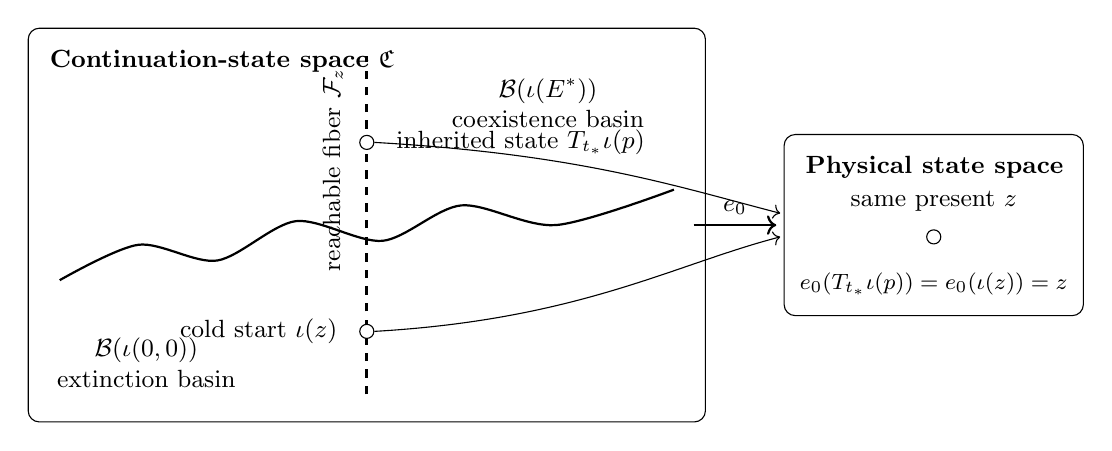
\begin{tikzpicture}[
  x=1cm,y=1cm,
  every node/.style={font=\small},
  state/.style={circle,draw,fill=white,inner sep=1.8pt},
  lab/.style={align=center}
]
  % Continuation-state space
  \draw[rounded corners] (0,0) rectangle (8.6,5.0);
  \node[anchor=north west,font=\small\bfseries] at (0.15,4.85)
    {Continuation-state space \(\mathfrak C\)};

  % Basin separator and labels
  \draw[thick] plot[smooth] coordinates {
    (0.4,1.8) (1.4,2.25) (2.4,2.05) (3.4,2.55)
    (4.5,2.30) (5.5,2.75) (6.7,2.50) (8.2,2.95)
  };
  \node[lab] at (1.5,0.75) {\(\mathcal B(\iota(0,0))\)\\extinction basin};
  \node[lab] at (6.6,4.05) {\(\mathcal B(\iota(E^*))\)\\coexistence basin};

  % Present-state fiber
  \draw[dashed,very thick] (4.3,0.35) -- (4.3,4.65);
  \node[anchor=south,rotate=90] at (4.12,3.2)
    {reachable fiber \(\mathcal F_z\)};

  % Two states in same fiber
  \node[state] (cold) at (4.3,1.15) {};
  \node[anchor=east] at (4.05,1.15)
    {cold start \(\iota(z)\)};

  \node[state] (inh) at (4.3,3.55) {};
  \node[anchor=west] at (4.55,3.55)
    {inherited state \(T_{t_*}\iota(p)\)};

  % Physical state space at right
  \draw[rounded corners] (9.6,1.35) rectangle (13.4,3.65);
  \node[anchor=north west,font=\small\bfseries] at (9.75,3.5)
    {Physical state space};
  \node[state] (z) at (11.5,2.35) {};
  \node[anchor=south] at (11.5,2.55)
    {same present \(z\)};

  % Evaluation projection
  \draw[->,thick] (8.45,2.5) -- node[above] {\(e_0\)} (9.5,2.5);
  \draw[->,thin] (inh.east) .. controls (7.0,3.4) and (8.2,3.0) .. (9.55,2.65);
  \draw[->,thin] (cold.east) .. controls (7.0,1.3) and (8.2,2.0) .. (9.55,2.35);

  % Caption-like logical statement within figure
  \node[align=center,font=\footnotesize] at (11.5,1.75)
    {\(e_0(T_{t_*}\iota(p))=e_0(\iota(z))=z\)};
\end{tikzpicture}
}
  \caption{Geometry of a multibasin reachable present-state fiber.  The inherited continuation state and the canonical cold start have the identical present evaluation \(z\), but lie in different basins in the continuation-state space.  The diagram is schematic; the existence of this configuration is proved in \cref{thm:principal}.}
  \label{fig:fiber-geometry}
\end{figure}

\begin{proposition}[Physical convergence lifts to continuation-state convergence]
\label{prop:physical-to-continuation}
Let \(X(\cdot;p)\) be the standard point-IVP solution of \eqref{eq:caputo-general}. If
\[
  X(t;p)\to X^*,
  \qquad
  g(X^*)=0,
\]
then
\[
  T_t\iota(p)\to\iota(X^*)
\]
in the compact-open topology of \(\Cspace\).
\end{proposition}

\begin{proof}
Fix \(N>0\) and \(0\le\eta\le N\). By the continuation-state formula,
\[
  (T_t\iota(p))(\eta)
  =
  p+
  \frac{1}{\Gamma(\alpha)}
  \int_0^t
  (t+\eta-s)^{\alpha-1}g(X(s;p))\,ds.
\]
On the other hand,
\[
  X(t+\eta;p)
  =
  p+
  \frac{1}{\Gamma(\alpha)}
  \int_0^{t+\eta}
  (t+\eta-s)^{\alpha-1}g(X(s;p))\,ds.
\]
Subtracting gives
\begin{align*}
  (T_t\iota(p))(\eta)-X^*
  &=
  X(t+\eta;p)-X^* \\
  &\quad-
  \frac{1}{\Gamma(\alpha)}
  \int_t^{t+\eta}
  (t+\eta-s)^{\alpha-1}g(X(s;p))\,ds.
\end{align*}
The first term tends uniformly to zero for \(0\le\eta\le N\). The second satisfies
\[
  \sup_{0\le\eta\le N}
  \left\|
  \frac{1}{\Gamma(\alpha)}
  \int_t^{t+\eta}
  (t+\eta-s)^{\alpha-1}g(X(s;p))\,ds
  \right\|
  \le
  \frac{N^\alpha}{\Gamma(\alpha+1)}
  \sup_{s\ge t}\|g(X(s;p))\|,
\]
which also tends to zero because \(g(X(t;p))\to g(X^*)=0\). Hence
\[
  \sup_{0\le\eta\le N}
  \|(T_t\iota(p))(\eta)-X^*\|\to0
\]
for every \(N\), which is compact-open convergence.
\end{proof}

\begin{proposition}[Basin-entry criterion]
\label{prop:basin-entry}
Let \(A_-\neq A_+\) be invariant asymptotic states or attractors in \(\Cspace\). Suppose
\[
  \iota(U_-)\subset\Basin(A_-),
  \qquad
  \iota(p)\in\Basin(A_+),
\]
for a physical set \(U_-\subset X_{\mathrm{phys}}\). If
\[
  z=X(t_*;p)\in U_-,
\]
then
\[
  T_{t_*}\iota(p),\ \iota(z)\in\Fiber{z},
\]
with
\[
  T_{t_*}\iota(p)\in\Basin(A_+),
  \qquad
  \iota(z)\in\Basin(A_-).
\]
Consequently \(\Fiber{z}\) is multibasin.
\end{proposition}

\begin{proof}
The two states have the same present value:
\[
  e_0(T_{t_*}\iota(p))
  =
  X(t_*;p)
  =
  z
  =
  e_0(\iota(z)).
\]
Both belong to \(\Reach\), so both lie in \(\Fiber{z}\). Basin positive invariance gives
\[
  T_{t_*}\iota(p)\in\Basin(A_+),
\]
while the definition of \(U_-\) gives
\[
  \iota(z)\in\Basin(A_-).
\]
Since \(A_-\neq A_+\), the fiber intersects two distinct basins.
\end{proof}

\begin{corollary}[Nondegenerate time-interval criterion]
\label{cor:time-interval}
Under the hypotheses of \cref{prop:basin-entry}, if
\[
  X(t;p)\in U_-
  \qquad
  \text{for every }t\in I
\]
on a nondegenerate interval \(I\), then
\[
  \Fiber{X(t;p)}
\]
is multibasin for every \(t\in I\).
\end{corollary}

\begin{remark}[Why compact-open topology is essential]
\label{rem:tail-anchoring}
For any fixed \(T>0\), if \(X(\cdot;p)\) is bounded on \([0,T]\), then
\[
  (T_T\iota(p))(\tau)
  =
  p+
  \frac{1}{\Gamma(\alpha)}
  \int_0^T
  (T+\tau-s)^{\alpha-1}g(X(s;p))\,ds
  \to p
\]
as \(\tau\to\infty\). Thus a finite-time continuation state need not be globally close to a terminal equilibrium in the unweighted sup norm, even when the underlying physical trajectory converges. The compact-open topology is therefore not a technical convenience but a structural feature of the continuation-state representation.
\end{remark}

\section{A scalar purity contrast}
\label{sec:scalar-purity}

The multibasin-fiber mechanism is not automatic in fractional dynamics. In a broad scalar threshold class, the current scalar value still determines the basin label on the physically reachable state set.

\begin{theorem}[Scalar equilibrium-partition fiber purity]
\label{thm:scalar-purity}
Consider the scalar autonomous Caputo equation
\[
  \CapD x=g(x).
\]
Assume that:
\begin{enumerate}[label=(S\arabic*)]
  \item equilibrium values are barriers for non-equilibrium standard trajectories;
  \item every connected component of the physical domain between consecutive equilibrium values has one asymptotic basin label;
  \item equilibrium lifts are stationary and no non-equilibrium standard trajectory reaches an equilibrium at positive time.
\end{enumerate}
Then every physically reachable present-state fiber is basin-pure.
\end{theorem}

\begin{proof}
Let
\[
  \phi=T_t\iota(x_0)\in\Fiber{x}.
\]
If \(x\) lies in one of the open components between consecutive equilibrium values, the barrier property implies that \(x_0\) and \(x\) lie in the same component. By hypothesis, \(\iota(x_0)\) has the unique basin label assigned to that component, and basin positive invariance gives the same label to
\[
  T_t\iota(x_0)=\phi.
\]
Because \(\phi\) was arbitrary, the entire fiber is basin-pure.

If \(x\) itself is an equilibrium value, finite-time nonattainment forces \(x_0=x\), and stationarity gives
\[
  \Fiber{x}=\{\iota(x)\}.
\]
\end{proof}

For the scalar strong-Allee equation
\begin{equation}
  \CapD x=x(1-x)(x-\theta),
  \qquad
  0<\theta<1,
  \label{eq:scalar-allee}
\end{equation}
published Caputo attractor and separation results
\cite{AreaNieto2023AlleeCaputo,DoanKloeden2022Attractors,CongTuan2017}
give the positive-domain classification
\[
  0<x<\theta
  \Longrightarrow
  \Fiber{x}\subset\Basin(\iota(0)),
\]
and
\[
  x>\theta
  \Longrightarrow
  \Fiber{x}\subset\Basin(\iota(1)).
\]
Thus the basin split proved later is not a generic consequence of fractional memory alone; it requires genuinely coupled multidimensional dynamics.

\section{Strong-Allee dynamics and analytic basin certificates}
\label{sec:model}

Writing the physical vector state as
\[
  X(t)=(x(t),y(t)),
\]
we consider
\begin{subequations}
\label{eq:model}
\begin{align}
  \CapD x
  &=
  x(1-x)(x-\theta)-axy,
  \label{eq:model-x}\\
  \CapD y
  &=
  y(bx-m),
  \label{eq:model-y}
\end{align}
\end{subequations}
with
\[
  0<\alpha<1,
  \qquad
  a,b,m>0,
  \qquad
  0<\theta<1.
\]
The underlying ecological vector field has been studied previously at integer order
\cite{YeEtAl2019StrongAlleePredatorPrey}; here it serves as a transparent positive system in which continuation-state basin geometry can be resolved rigorously.

If
\[
  \theta<\frac{m}{b}<1,
\]
the positive coexistence equilibrium is
\begin{equation}
  \Eeq=(x^*,y^*),
  \qquad
  x^*=\frac{m}{b},
  \qquad
  y^*=\frac{(1-x^*)(x^*-\theta)}{a}.
  \label{eq:coexistence-equilibrium}
\end{equation}
The Jacobian at \(\Eeq\) is
\begin{equation}
  J=
  \begin{pmatrix}
    x^*(1+\theta-2x^*) & -ax^*\\
    by^* & 0
  \end{pmatrix}.
  \label{eq:coexistence-jacobian}
\end{equation}

\subsection{Cold-start extinction}

\begin{theorem}[Cold-start extinction strip]
\label{thm:extinction-strip}
Assume
\[
  \theta<\frac{m}{b}
\]
and define
\begin{equation}
  \Ext
  =
  \{(x,y):0<x<\theta,\ y\ge0\}.
  \label{eq:extinction-strip}
\end{equation}
Then every standard point initial condition in \(\Ext\) generates a global nonnegative solution satisfying
\[
  X(t)\to(0,0).
\]
Equivalently,
\[
  \iota(\Ext)\subset\Basin(\iota(0,0)).
\]
\end{theorem}

\begin{proof}
The vector field is locally Lipschitz and quasi-positive on the coordinate axes. Caputo viability and extremum results
\cite{GirejkoMozyrskaWyrwas2011Viability,AlRefai2012ExtremePoints}
therefore preserve the nonnegative cone.

Let \(u\) solve
\[
  \CapD u=u(1-u)(u-\theta),
  \qquad
  u(0)=x_0.
\]
Since \(y(t)\ge0\),
\[
  \CapD x
  \le
  x(1-x)(x-\theta).
\]
The scalar comparison principle \cite{Wu2020Comparison} yields
\[
  0\le x(t)\le u(t).
\]
For \(0<x_0<\theta\), the scalar strong-Allee solution remains below \(\theta\) and converges to zero, hence
\[
  x(t)\to0
  \qquad\text{and}\qquad
  x(t)<\theta.
\]

Set
\[
  \delta=m-b\theta>0.
\]
Then
\[
  \CapD y
  =
  y(bx-m)
  \le
  -\delta y.
\]
Comparison with
\[
  \CapD v=-\delta v,
  \qquad
  v(0)=y_0,
\]
gives
\[
  0\le y(t)\le y_0E_\alpha(-\delta t^\alpha)\to0.
\]
The resulting bounds exclude finite-time blow-up by the continuation theorem of Wu and Liu
\cite{WuLiu2020Continuation}. Therefore the solution is global and tends to \((0,0)\).
\end{proof}

\subsection{Inherited-memory survival}

A late physical near-hit to \(\Eeq\) is not a valid survival proof for a Caputo trajectory because restarting at that physical point discards the inherited memory. We therefore retain the entire prehistory explicitly.

Write
\[
  U=X-\Eeq
\]
and
\begin{equation}
  \CapD U=JU+N(U).
  \label{eq:linearized-system}
\end{equation}
Fix a vector norm \(\|\cdot\|\) and its induced matrix norm. Define
\[
  \Psi_J(t)
  =
  t^{\alpha-1}E_{\alpha,\alpha}(Jt^\alpha).
\]
Under the Matignon sector condition, stable Mittag--Leffler estimates imply
\[
  K_J
  :=
  \int_0^\infty\|\Psi_J(s)\|\,ds
  <\infty
\]
\cite{CongDoanTuan2017Perron,CongTuanTrinh2020Asymptotic,Becker2011WeaklySingularResolvents}.

\begin{theorem}[Memory-tail survival criterion]
\label{thm:memory-tail}
Let \(U(t)\) be a solution of \eqref{eq:linearized-system} whose history is known on \([0,T]\). Suppose that, for some \(r>0\),
\[
  \|N(U)\|
  \le
  C_r\|U\|^2
  \qquad
  (\|U\|\le r).
\]
For a finite cut \(T\), define
\begin{equation}
  v_T(t)
  =
  E_\alpha(Jt^\alpha)U_0
  +
  \int_0^T
  \Psi_J(t-s)N(U(s))\,ds,
  \qquad t\ge T,
  \label{eq:memory-response}
\end{equation}
and
\[
  M_T
  =
  \sup_{t\ge T}\|v_T(t)\|.
\]
If
\begin{equation}
  M_T+K_JC_rr^2<r,
  \label{eq:M1}
\end{equation}
then
\[
  U(t)\to0.
\]
\end{theorem}

\begin{proof}
Variation of constants gives the exact split
\begin{equation}
  U(t)
  =
  v_T(t)
  +
  \int_T^t
  \Psi_J(t-s)N(U(s))\,ds.
  \label{eq:exact-memory-split}
\end{equation}
This is a decomposition of the original trajectory, not a restart at time \(T\).

If \(t_e\) were a first exit from the radius-\(r\) ball after \(T\), then
\[
  \|U(t_e)\|
  \le
  M_T+
  \int_T^{t_e}
  \|\Psi_J(t_e-s)\|C_rr^2\,ds
  \le
  M_T+K_JC_rr^2<r,
\]
a contradiction. Hence the trajectory remains in the ball.

Inside the ball,
\[
  \|N(U)\|\le C_rr\|U\|,
\]
and \eqref{eq:M1} implies
\[
  K_JC_rr<1.
\]
The term \(v_T(t)\) tends to zero: the homogeneous term decays by Mittag--Leffler stability, while the finite-history convolution in \eqref{eq:memory-response} tends to zero because \(\Psi_J(t-s)\to0\) for each fixed \(s\in[0,T]\).

Set
\[
  L=\limsup_{t\to\infty}\|U(t)\|.
\]
Splitting the nonlinear convolution in \eqref{eq:exact-memory-split} at a large fixed time and using \(\Psi_J\in L^1(\mathbb{R}_+)\) gives
\[
  L\le K_JC_rr\,L.
\]
Since \(K_JC_rr<1\), one obtains \(L=0\).
\end{proof}

\section{Certified same-present basin splitting}
\label{sec:principal-theorem}

We now fix the exact rational benchmark
\begin{equation}
  \alpha=\frac{17}{20},
  \qquad
  \theta=\frac12,
  \qquad
  a=\frac12,
  \qquad
  b=1,
  \qquad
  m=\frac45,
  \label{eq:B215-parameters}
\end{equation}
with standard initial point
\begin{equation}
  p=
  \left(
  \frac{277}{100},
  \frac{467}{1000}
  \right).
  \label{eq:B215-p}
\end{equation}
The coexistence equilibrium is
\begin{equation}
  \Eeq=
  \left(
  \frac45,\frac3{25}
  \right).
  \label{eq:B215-E}
\end{equation}
At \(\Eeq\),
\begin{equation}
  J=
  \begin{pmatrix}
    -\frac2{25} & -\frac25\\[1mm]
    \frac3{25} & 0
  \end{pmatrix},
  \label{eq:B215-J}
\end{equation}
with eigenvalues
\[
  \lambda_\pm
  =
  \frac{-1\pm i\sqrt{29}}{25}.
\]
Thus the Matignon sector condition holds for \(\alpha=17/20\).

Writing
\[
  U=(\xi,\eta)=X-\Eeq,
\]
the nonlinear remainder in \eqref{eq:linearized-system} is
\begin{equation}
  N_1(\xi,\eta)
  =
  -\frac9{10}\xi^2
  -\frac12\xi\eta
  -\xi^3,
  \qquad
  N_2(\xi,\eta)=\xi\eta.
  \label{eq:B215-remainder}
\end{equation}

\begin{proposition}[Certified finite excursion]
\label{prop:certified-entry}
Under the arithmetic model stated in \cref{sec:cap}, the exact solution of \eqref{eq:model}--\eqref{eq:B215-p} is uniquely enclosed on \([0,300]\), with physical-state error at most
\[
  2.2193\times10^{-4}.
\]
Moreover,
\begin{equation}
  0<x(t)<\frac12,
  \qquad
  y(t)>0
  \qquad
  \text{for every }
  t\in I_*,
  \label{eq:entry-whole-interval}
\end{equation}
where
\begin{equation}
  I_*=
  [5.8576774143,\ 13.7275388580].
  \label{eq:Istar}
\end{equation}
\end{proposition}

\begin{proof}
This is the finite-history certificate established in \cref{sec:cap}; see in particular \cref{tab:certificate-summary}.
\end{proof}

\begin{proposition}[Certified survival of the same standard orbit]
\label{prop:certified-survival}
For the same exact standard IVP, the memory-tail quantities at \(T=300\) satisfy
\[
  K_J\le11.3499043,
  \qquad
  M_T\le0.043232414,
\]
and
\[
  C_r\le0.3695518+0.1627353\,r.
\]
At
\[
  r=\frac{2221}{20000},
\]
one has
\begin{equation}
  r-K_JC_rr^2-M_T
  \ge
  0.0135626>0,
  \label{eq:B215-M1-margin}
\end{equation}
with
\[
  K_JC_rr\le0.48857<1.
\]
Consequently,
\[
  X(t;p)\to\Eeq.
\]
\end{proposition}

\begin{proof}
The bounds are certified in \cref{sec:cap}. Inequality \eqref{eq:B215-M1-margin} is exactly the hypothesis of \cref{thm:memory-tail}.
\end{proof}

\begin{theorem}[Multibasin reachable present-state fibers]
\label{thm:principal}
For the exact Caputo system \eqref{eq:model} with parameters \eqref{eq:B215-parameters} and initial point \eqref{eq:B215-p}, fix any
\[
  t_*\in I_*,
\]
and define
\[
  z_*=X(t_*;p).
\]
Then
\begin{equation}
  \Fiber{z_*}\cap\Basin(\iota(0,0))
  \neq\varnothing,
  \qquad
  \Fiber{z_*}\cap\Basin(\iota(\Eeq))
  \neq\varnothing.
  \label{eq:multibasin-conclusion}
\end{equation}
More precisely,
\[
  \iota(z_*)\in\Basin(\iota(0,0)),
\]
whereas
\[
  T_{t_*}\iota(p)\in\Basin(\iota(\Eeq)),
\]
although
\begin{equation}
  e_0(\iota(z_*))
  =
  e_0(T_{t_*}\iota(p))
  =
  z_*.
  \label{eq:same-present}
\end{equation}
\end{theorem}

\begin{proof}
By \cref{prop:certified-entry},
\[
  z_*\in\Ext.
\]
Hence \cref{thm:extinction-strip} gives
\[
  \iota(z_*)\in\Basin(\iota(0,0)).
\]

By \cref{prop:certified-survival},
\[
  X(t;p)\to\Eeq.
\]
Then \cref{prop:physical-to-continuation} implies
\[
  T_t\iota(p)\to\iota(\Eeq),
\]
so
\[
  \iota(p)\in\Basin(\iota(\Eeq)).
\]
Positive invariance yields
\[
  T_{t_*}\iota(p)\in\Basin(\iota(\Eeq)).
\]
Finally, \eqref{eq:same-present} shows that the inherited continuation state and the canonical cold start lie in the same reachable present-state fiber. Applying \cref{prop:basin-entry} proves \eqref{eq:multibasin-conclusion}.
\end{proof}

\begin{corollary}[A nondegenerate interval of certified basin splits]
\label{cor:principal-interval}
For every \(t\in I_*\), the reachable present-state fiber
\[
  \Fiber{X(t;p)}
\]
is multibasin.
\end{corollary}

\begin{remark}[Scope of the conclusion]
\label{rem:scope-principal}
\Cref{cor:principal-interval} is indexed by a nondegenerate interval of physical time. We do not require, and do not currently claim, that
\[
  t\mapsto X(t;p)
\]
is injective on \(I_*\). Thus the theorem does not rely on a topological arc of distinct physical states.
\end{remark}

\section{Computer-assisted validation}
\label{sec:cap}

The proof of \cref{thm:principal} requires two finite-time facts about the same exact rational point IVP: the trajectory must be enclosed tightly enough to certify entry into the cold-start extinction strip, and the validated finite history must be accurate enough to certify the inherited memory term in \cref{thm:memory-tail}. A direct normwise fractional Grönwall estimate is too pessimistic for this orbit because it replaces the time-dependent matrix dynamics by absolute-value amplification. We therefore validate the computed trajectory by an orbit-linearized Volterra fixed-point argument.

\begin{figure}[t]
  \centering
  \resizebox{\textwidth}{!}{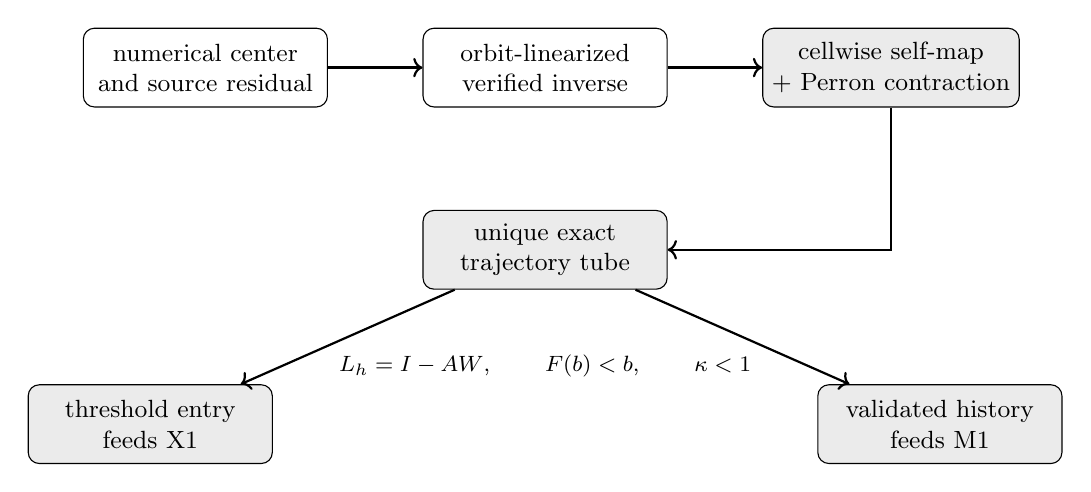
\begin{tikzpicture}[
  node distance=8mm and 12mm,
  box/.style={draw,rounded corners,align=center,minimum height=10mm,minimum width=31mm,font=\small},
  cert/.style={draw,rounded corners,align=center,minimum height=10mm,minimum width=31mm,font=\small,fill=black!8},
  arr/.style={->,thick}
]
  \node[box] (center) {numerical center\\and source residual};
  \node[box,right=of center] (inv) {orbit-linearized\\verified inverse};
  \node[cert,right=of inv] (close) {cellwise self-map\\+\ Perron contraction};

  \node[cert,below=13mm of inv] (tube) {unique exact\\trajectory tube};

  \node[cert,below left=12mm and 19mm of tube] (entry)
    {threshold entry\\feeds X1};
  \node[cert,below right=12mm and 19mm of tube] (tail)
    {validated history\\feeds M1};

  \draw[arr] (center)--(inv);
  \draw[arr] (inv)--(close);
  \draw[arr] (close.south) |- (tube.east);
  \draw[arr] (tube)--(entry);
  \draw[arr] (tube)--(tail);

  \node[font=\footnotesize,align=center,below=7mm of tube]
    {\(L_h=I-AW\), \qquad \(F(b)<b\), \qquad \(\kappa<1\)};
\end{tikzpicture}
}
  \caption{Logical architecture of the finite-history computer-assisted proof.  The sign-aware inverse is validated before nonnegative cellwise bounds are applied; the resulting exact state tube is then used independently for threshold entry and for the memory-tail constants.}
  \label{fig:cap-architecture}
\end{figure}

\subsection{Source correction equation}

Let the numerical center be written as
\[
  \widehat X(t)
  =
  p+I^\alpha\phi(t),
\]
where
\[
  (I^\alpha f)(t)
  =
  \frac1{\Gamma(\alpha)}
  \int_0^t(t-s)^{\alpha-1}f(s)\,ds.
\]
Define
\[
  \rho(t)
  =
  \phi(t)-g(\widehat X(t)).
\]
If
\[
  X=\widehat X+I^\alpha f,
\]
then the exact correction source \(f\) satisfies
\begin{equation}
  \mathcal H(f)
  =
  f-
  \left[
  g(\widehat X+I^\alpha f)-g(\widehat X)
  \right]
  +\rho
  =
  0.
  \label{eq:source-equation}
\end{equation}
At \(f=0\),
\[
  D\mathcal H(0)=I-K,
  \qquad
  (Kf)(t)=A(t)I^\alpha f(t),
\]
with
\[
  A(t)=Dg(\widehat X(t)).
\]

\subsection{Discrete inverse}

Let
\[
  0=t_0<t_1<\cdots<t_N=T
\]
be the adaptive mesh and let \(\pi\) denote continuous piecewise-linear interpolation at the nodes. The fractional integral of the hat basis produces a lower-triangular block matrix \(W\). In the source variable, the projected derivative is
\begin{equation}
  L_h=I-AW.
  \label{eq:source-discrete-operator}
\end{equation}
The ordering \(AW\), rather than \(WA\), follows directly from \(Kf=A I^\alpha f\).

A numerical inverse \(\widetilde R\) is computed by block forward substitution and its residual
\[
  E=I-L_h\widetilde R
\]
is enclosed. For the primary certificate
\[
  T=300,
  \qquad
  N=12000,
\]
the verified residual satisfies
\begin{equation}
  \|E\|_\infty
  \le
  2.09\times10^{-10}.
  \label{eq:inverse-residual}
\end{equation}
A Neumann argument therefore verifies invertibility of \(L_h\).

Define the continuous inverse model
\[
  B=L_h^{-1}\pi+(I-\pi).
\]
On the complementary piecewise-linear and interpolation-bubble subspaces,
\[
  B^{-1}=L_h\pi+(I-\pi),
\]
so \(B\) is injective. Hence a fixed point of
\[
  \mathcal T(f)=f-B\mathcal H(f)
\]
is a zero of \(\mathcal H\), not merely a zero of \(B\mathcal H\).

The analytic background for weakly singular Volterra resolvents and collocation, together with rigorous approximate-inverse fixed-point methods, is well established
\cite{Becker2011WeaklySingularResolvents,BrunnerPedasVainikko1999WeaklySingularCollocation,LiangBrunner2019WeaklySingularCollocation,BredenLessard2018PolynomialCAP,ChurchQueirolo2024HopfCAP}. These ingredients are used here as proof machinery rather than as the principal contribution.

\subsection{Cellwise positive self-map}

For each mesh cell
\[
  C_n=[t_n,t_{n+1}],
\]
we track three nonnegative source bounds:
\[
  \omega_n
  \ge
  \sup_{t\in C_n}|f(t)|,
\]
\[
  \vartheta_n
  \ge
  \operatorname{osc}_{C_n}f,
\]
and
\[
  \beta_n
  \ge
  \sup_{t\in C_n}|(I-\pi)f(t)|.
\]
Collect them into
\[
  b=(\omega,\vartheta,\beta).
\]
The Newton-like map admits a componentwise monotone upper-bound operator
\begin{equation}
  F(b)
  =
  Y+Mb+Q_2(b),
  \label{eq:positive-bound-map}
\end{equation}
where \(Y\) bounds the propagated residual, \(M\) the orbit-linearized interpolation terms, and \(Q_2\) the nonlinear derivative remainder.

The primary certificate verifies
\begin{equation}
  F(b)<b
  \label{eq:self-map-vector}
\end{equation}
on all \(3N=36000\) component inequalities, with minimum relative slack
\begin{equation}
  6.036\times10^{-4}.
  \label{eq:self-map-slack}
\end{equation}
Thus the closed cellwise set determined by the sup, oscillation, and interpolation-bubble bounds is mapped strictly into itself.

A conventional one-radius scalar radii inequality does not close for this orbit. The proof therefore uses the stronger vector inequality \eqref{eq:self-map-vector}, which retains temporal localization instead of collapsing all cells into one radius.

\subsection{Perron-weighted contraction}

Let
\[
  q=(q^{\mathrm{sup}},q^{\mathrm{osc}},q^{\mathrm{bub}})
\]
be strictly positive weights obtained from the positive derivative-bound operator. Define
\[
  \|h\|_q
  =
  \max\left\{
  \max_n\frac{\sup_{C_n}|h|}{q_n^{\mathrm{sup}}},
  \max_n\frac{\operatorname{osc}_{C_n}h}{q_n^{\mathrm{osc}}},
  \max_n\frac{\sup_{C_n}|(I-\pi)h|}{q_n^{\mathrm{bub}}}
  \right\}.
\]
Because the mesh is finite and every weight is positive, \(\|\cdot\|_q\) is equivalent to the sup topology on the continuous source space. The closed self-map set is therefore complete.

The derivative bounds verify
\begin{equation}
  \operatorname{Lip}_{\|\cdot\|_q}
  (\mathcal T)
  \le
  \kappa,
  \qquad
  \kappa\le0.083612<1.
  \label{eq:Perron-contraction}
\end{equation}
Banach's fixed-point theorem yields a unique correction source \(f^*\), and injectivity of \(B\) gives
\[
  \mathcal H(f^*)=0.
\]
Consequently
\[
  X(t)=\widehat X(t)+I^\alpha f^*(t)
\]
is the exact Caputo solution on \([0,300]\).

\subsection{Validated state tube and threshold entry}

Propagating the source enclosure through \(I^\alpha\) gives
\[
  \sup_{0\le t\le300}
  \|X(t)-\widehat X(t)\|_{\mathrm{adapted}}
  \le
  4.8661\times10^{-4},
\]
and
\begin{equation}
  \sup_{0\le t\le300}
  \|X(t)-\widehat X(t)\|_2
  \le
  2.2193\times10^{-4}.
  \label{eq:physical-tube}
\end{equation}
Adding this certified pad to the cellwise state enclosure proves \eqref{eq:entry-whole-interval}. A representative interior cell is
\[
  t\in[8.9839195370,\ 8.9927932624],
\]
where
\[
  x\in[0.468938793,\ 0.469058899],
  \qquad
  y\ge0.248262346.
\]
Thus the prey threshold is crossed with certified margin
\[
  \frac12-x_{\max}
  \ge
  0.0309411007.
\]

\subsection{Memory-tail quantities and redundant cut}

The same validated finite history is inserted into the exact memory-tail representation \eqref{eq:memory-response}. The resulting primary and redundant proof constants are summarized in \cref{tab:certificate-summary}.

\begin{table}[t]
\centering
\caption{Primary and independent redundant certificates for the exact B215 trajectory. The \(T=300\) computation is used in the theorem proof; \(T=1000\) is retained as robustness redundancy.}
\label{tab:certificate-summary}
\begin{tabular}{lcc}
\toprule
Quantity & \(T=300,\ N=12000\) & \(T=1000,\ N=20000\)\\
\midrule
self-map min. relative slack
& \(6.036\times10^{-4}\)
& \(5.651\times10^{-4}\)\\
Perron contraction \(\kappa\)
& \(\le0.083612\)
& \(\le0.187495\)\\
physical state tube
& \(\le2.2193\times10^{-4}\)
& \(\le1.9773\times10^{-3}\)\\
\(K_J\)
& \(\le11.3499043\)
& \(\le11.3457429\)\\
\(M_T\)
& \(\le0.043232414\)
& \(\le0.015478583\)\\
M1 margin
& \(\ge0.0135626\)
& \(\ge0.0413364\)\\
\bottomrule
\end{tabular}
\end{table}

For the primary cut,
\[
  r=\frac{2221}{20000},
\]
and the certified values yield \eqref{eq:B215-M1-margin}. The independent cut at \(T=1000\) is not logically needed for \cref{thm:principal}; it is included to demonstrate that the basin classification is not an artifact of one particular cut time.

\begin{figure}[t]
  \centering
  \resizebox{\textwidth}{!}{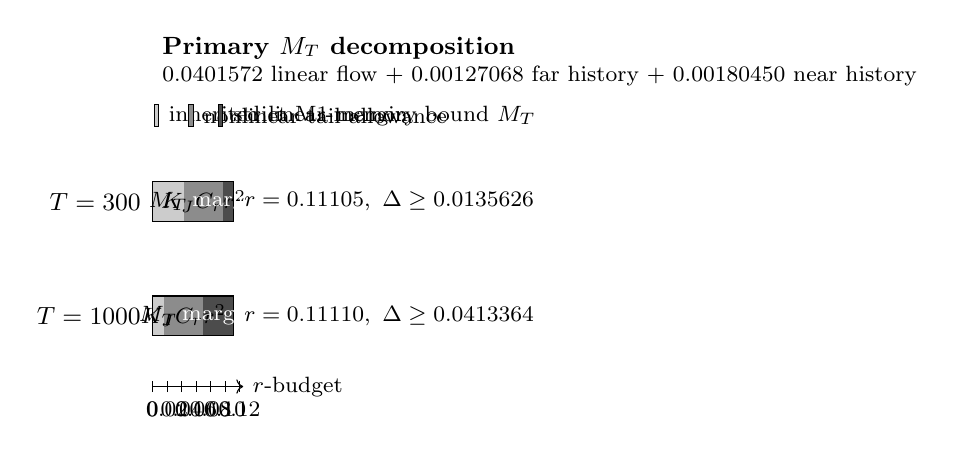
\begin{tikzpicture}[x=9.2cm,y=1cm,every node/.style={font=\footnotesize}]
  % axes
  \draw[->] (0,0.35) -- (0.125,0.35) node[anchor=west] {\(r\)-budget};
  \foreach \x/\lab in {0/0,0.02/0.02,0.04/0.04,0.06/0.06,0.08/0.08,0.10/0.10,0.12/0.12}{
    \draw (\x,0.28)--(\x,0.42);
    \node[below] at (\x,0.28) {\lab};
  }

  \node[anchor=east,font=\small\bfseries] at (-0.003,2.70) {\(T=300\)};
  \node[anchor=east,font=\small\bfseries] at (-0.003,1.25) {\(T=1000\)};

  % T=300 stacked bar
  \fill[black!20] (0,2.45) rectangle (0.0432324134,2.95);
  \fill[black!45] (0.0432324134,2.45) rectangle (0.0974873734,2.95);
  \fill[black!70] (0.0974873734,2.45) rectangle (0.11105,2.95);
  \draw (0,2.45) rectangle (0.11105,2.95);

  % T=1000 stacked bar
  \fill[black!20] (0,1.00) rectangle (0.0154785828,1.50);
  \fill[black!45] (0.0154785828,1.00) rectangle (0.0697636399,1.50);
  \fill[black!70] (0.0697636399,1.00) rectangle (0.11110,1.50);
  \draw (0,1.00) rectangle (0.11110,1.50);

  % labels on bars
  \node[align=center] at (0.0216,2.70) {\(M_T\)};
  \node[align=center] at (0.07036,2.70) {\(K_JC_rr^2\)};
  \node[align=center,text=white] at (0.10427,2.70) {margin};

  \node[align=center] at (0.00774,1.25) {\(M_T\)};
  \node[align=center] at (0.04262,1.25) {\(K_JC_rr^2\)};
  \node[align=center,text=white] at (0.09043,1.25) {margin};

  % numeric annotations
  \node[anchor=west] at (0.1130,2.70)
    {\(r=0.11105,\ \Delta\ge0.0135626\)};
  \node[anchor=west] at (0.1130,1.25)
    {\(r=0.11110,\ \Delta\ge0.0413364\)};

  % legend
  \draw[fill=black!20] (0.002,3.65) rectangle (0.008,3.93);
  \node[anchor=west] at (0.009,3.79) {inherited linear-memory bound \(M_T\)};
  \draw[fill=black!45] (0.050,3.65) rectangle (0.056,3.93);
  \node[anchor=west] at (0.057,3.79) {nonlinear tail allowance};
  \draw[fill=black!70] (0.091,3.65) rectangle (0.097,3.93);
  \node[anchor=west] at (0.098,3.79) {strict M1 margin};

  % term decomposition mini panel
  \node[anchor=west,font=\small\bfseries] at (0,4.65)
    {Primary \(M_T\) decomposition};
  \node[anchor=west] at (0,4.30)
    {\(0.0401572\) linear flow \(+\ 0.00127068\) far history \(+\ 0.00180450\) near history};
\end{tikzpicture}
}
  \caption{Certified memory-tail budgets for the primary and redundant cuts.  Each bar partitions the radius \(r\) into the inherited linear-memory term \(M_T\), the nonlinear tail allowance \(K_JC_rr^2\), and the remaining strict margin.  The top annotation gives the certified decomposition of \(M_T\) for the primary \(T=300\) proof.}
  \label{fig:memory-tail-budget}
\end{figure}

\subsection{Arithmetic model}
\label{subsec:arithmetic-model}

The current certificate combines exact-rational model data and Arb ball arithmetic with selected binary64 layers for the large \(O(N^2)\) matrix and positive-sum computations. The latter carry explicit operation-count and roundoff allowances. The TASK-0006 certificate additionally assumes a few-ulp model for selected elementary \texttt{libm} calls used in the large-kernel layer.

Accordingly, until the publication-hardening rerun is complete, the result is described as a \emph{computer-assisted theorem under the stated IEEE-754/libm arithmetic model}, rather than as an end-to-end interval-arithmetic proof. The arithmetic-hardening computation replaces the remaining load-bearing elementary-function evaluations by verified enclosures without changing the mathematical fixed-point argument.

\section{Geometry and interpretation}
\label{sec:geometry}

Theorem~\ref{thm:principal} can be read as a geometric statement about the projection
\[
  e_0:\Reach\to X_{\mathrm{phys}}.
\]
At a certified reached value
\[
  z_*=X(t_*;p),
  \qquad t_*\in I_*,
\]
the projection identifies two continuation states with the same present physical coordinates:
\[
  e_0(T_{t_*}\iota(p))
  =
  e_0(\iota(z_*))
  =
  z_*.
\]
Their basin labels nevertheless differ. The first state retains the entire nonlinear excursion from the original point initial condition and converges to coexistence; the second discards that history and, by \cref{thm:extinction-strip}, converges to extinction.

This distinction is stronger than the observation that fractional trajectories may intersect after projection onto physical coordinates. Such intersections are already known in fractional systems \cite{DeshpandeDaftardarGejjiVellaisamy2019}. What matters here is that the two physically reachable continuation states above the same present value have different asymptotic basin membership.

The closest conceptual analogue in hereditary dynamics occurs in dynamical-integrity methods for delay equations, where different histories sharing the same headpoint can evolve differently \cite{SzakszStepanHabib2024DynamicalIntegrity}. The present theorem adds a different ingredient: opposite asymptotic basin membership is proved for a physically reachable Caputo continuation state and the canonical cold start at exactly the same present value.

\subsection{Why the cold-start extinction strip does not classify the inherited state}

The set \(\Ext\) is a basin certificate only for the canonical embedding:
\[
  z\in\Ext
  \Longrightarrow
  \iota(z)\in\Basin(\iota(0,0)).
\]
It is not an invariant physical-state label for all continuation states above \(z\). Indeed, \cref{thm:principal} provides explicit states
\[
  T_{t_*}\iota(p)\in\Fiber{z_*}
\]
with \(z_*\in\Ext\) that lie instead in \(\Basin(\iota(\Eeq))\).

This observation also explains why a survival proof based on trapping the trajectory inside a physical-state region whose every cold start survives cannot prove the present phenomenon. The relevant survival certificate must depend on inherited memory. The memory-tail quantity \(v_T\) in \eqref{eq:memory-response} does exactly that: it absorbs the entire pre-\(T\) excursion before a local quadratic tail estimate is imposed.

\subsection{Why sign-aware validation matters}

A scalar normwise a posteriori bound treats the nonlinear excursion through absolute values and loses the rotations and cancellations of the matrix linearization
\[
  A(t)=Dg(\widehat X(t)).
\]
For the present benchmark, this produces artificial amplification many orders of magnitude larger than the response of the actual orbit-linearized Volterra operator.

The successful certificate therefore preserves the block-matrix signs in
\[
  L_h=I-AW
\]
and validates the inverse before applying nonnegative componentwise bounds to the remaining interpolation and nonlinear terms. This separation between a sign-aware linear inverse and a positive nonlinear enclosure is the practical reason the long excursion can be certified.

These diagnostics motivate the proof architecture, but they are not themselves part of the logical content of \cref{thm:principal}. The theorem depends only on the final validated self-map, contraction, threshold entry, and memory-tail inequalities.

\section{Discussion and limitations}
\label{sec:discussion}

\Cref{thm:principal} shows that basin membership in an autonomous Caputo system need not factor through the present physical coordinates, even when attention is restricted to physically reachable continuation states. The result is deliberately narrower than a generic statement that memory changes the future. History dependence is classical in hereditary dynamics, Caputo continuation-state representations are established, and fractional trajectory intersections are known. The point proved here is the simultaneous occurrence of:
\begin{enumerate}[label=(\roman*)]
  \item the identical current physical value;
  \item two physically reachable continuation states above that value;
  \item distinct asymptotic basin membership;
  \item a concrete extinction-versus-coexistence realization.
\end{enumerate}

A targeted literature audit did not identify a formally published theorem establishing this same-present-value, physically reachable Caputo basin split. We therefore position the contribution at that theorem-specific level rather than as a broad priority claim.

The ecological application should likewise be interpreted narrowly. Fractional predator--prey models with Allee effects, extinction/coexistence multistability, and basin calculations already have a substantial literature
\cite{RameshEtAl2025MemoryDoubleAllee,MondalEtAl2025Consequences,WangHan2025Allee,SahaEtAl2026AlleeBasin,PippalSati2026}. The vector field used here is also not new
\cite{YeEtAl2019StrongAlleePredatorPrey}. Its role is to supply a transparent positive system in which the continuation-state theorem can be proved.

Several limitations remain. First, the present result is an exact benchmark theorem, not yet an open-parameter persistence theorem. The strict threshold entry and the certified inequalities strongly suggest robustness, but a parameter-open result requires a separate quantitative persistence argument and is not claimed here. Second, \cref{cor:principal-interval} is indexed by a nondegenerate time interval; injectivity of \(t\mapsto X(t;p)\) on that interval is not part of the current certificate. Third, the computer-assisted proof currently uses a declared IEEE-754/libm arithmetic model in selected large-scale layers. The mathematical fixed-point argument is independent of that implementation choice, and a publication-hardening rerun is designed to replace the remaining load-bearing elementary-function evaluations by verified enclosures.

Finally, the distinction between physical-state basins and continuation-state basins suggests a broader methodological point. For nonlocal systems, a basin diagram drawn only in physical coordinates can conflate states that share the same present value but carry different inherited memory. The correct state space for asymptotic classification is the continuation space; physical coordinates are a projection of that geometry. The example proved here shows that this distinction can be dynamically decisive rather than merely formal.


\bibliographystyle{plain}
\bibliography{../bibliography/references}

\end{document}
